\chapter{Other Activities and Research}

\section*{Chennai Mathematical Institute (CMI)}

Seshadri founded CMI with Mathematics and Theoretical\break Computer Science. 
Even before IISERs came, Seshadri admitted into CMI talented students 
after school so that they can pursue their studies in an atmosphere of 
research. He wanted CMI to grow into a full-fledged University and as a 
first step wanted to have Physics. He asked me to help in Physics 
Faculty recruitment and teaching. I have been doing that. We now have a 
Theoretical Physics Group of outstanding young faculty members.
\medskip

\begin{figure}[h]
\centering
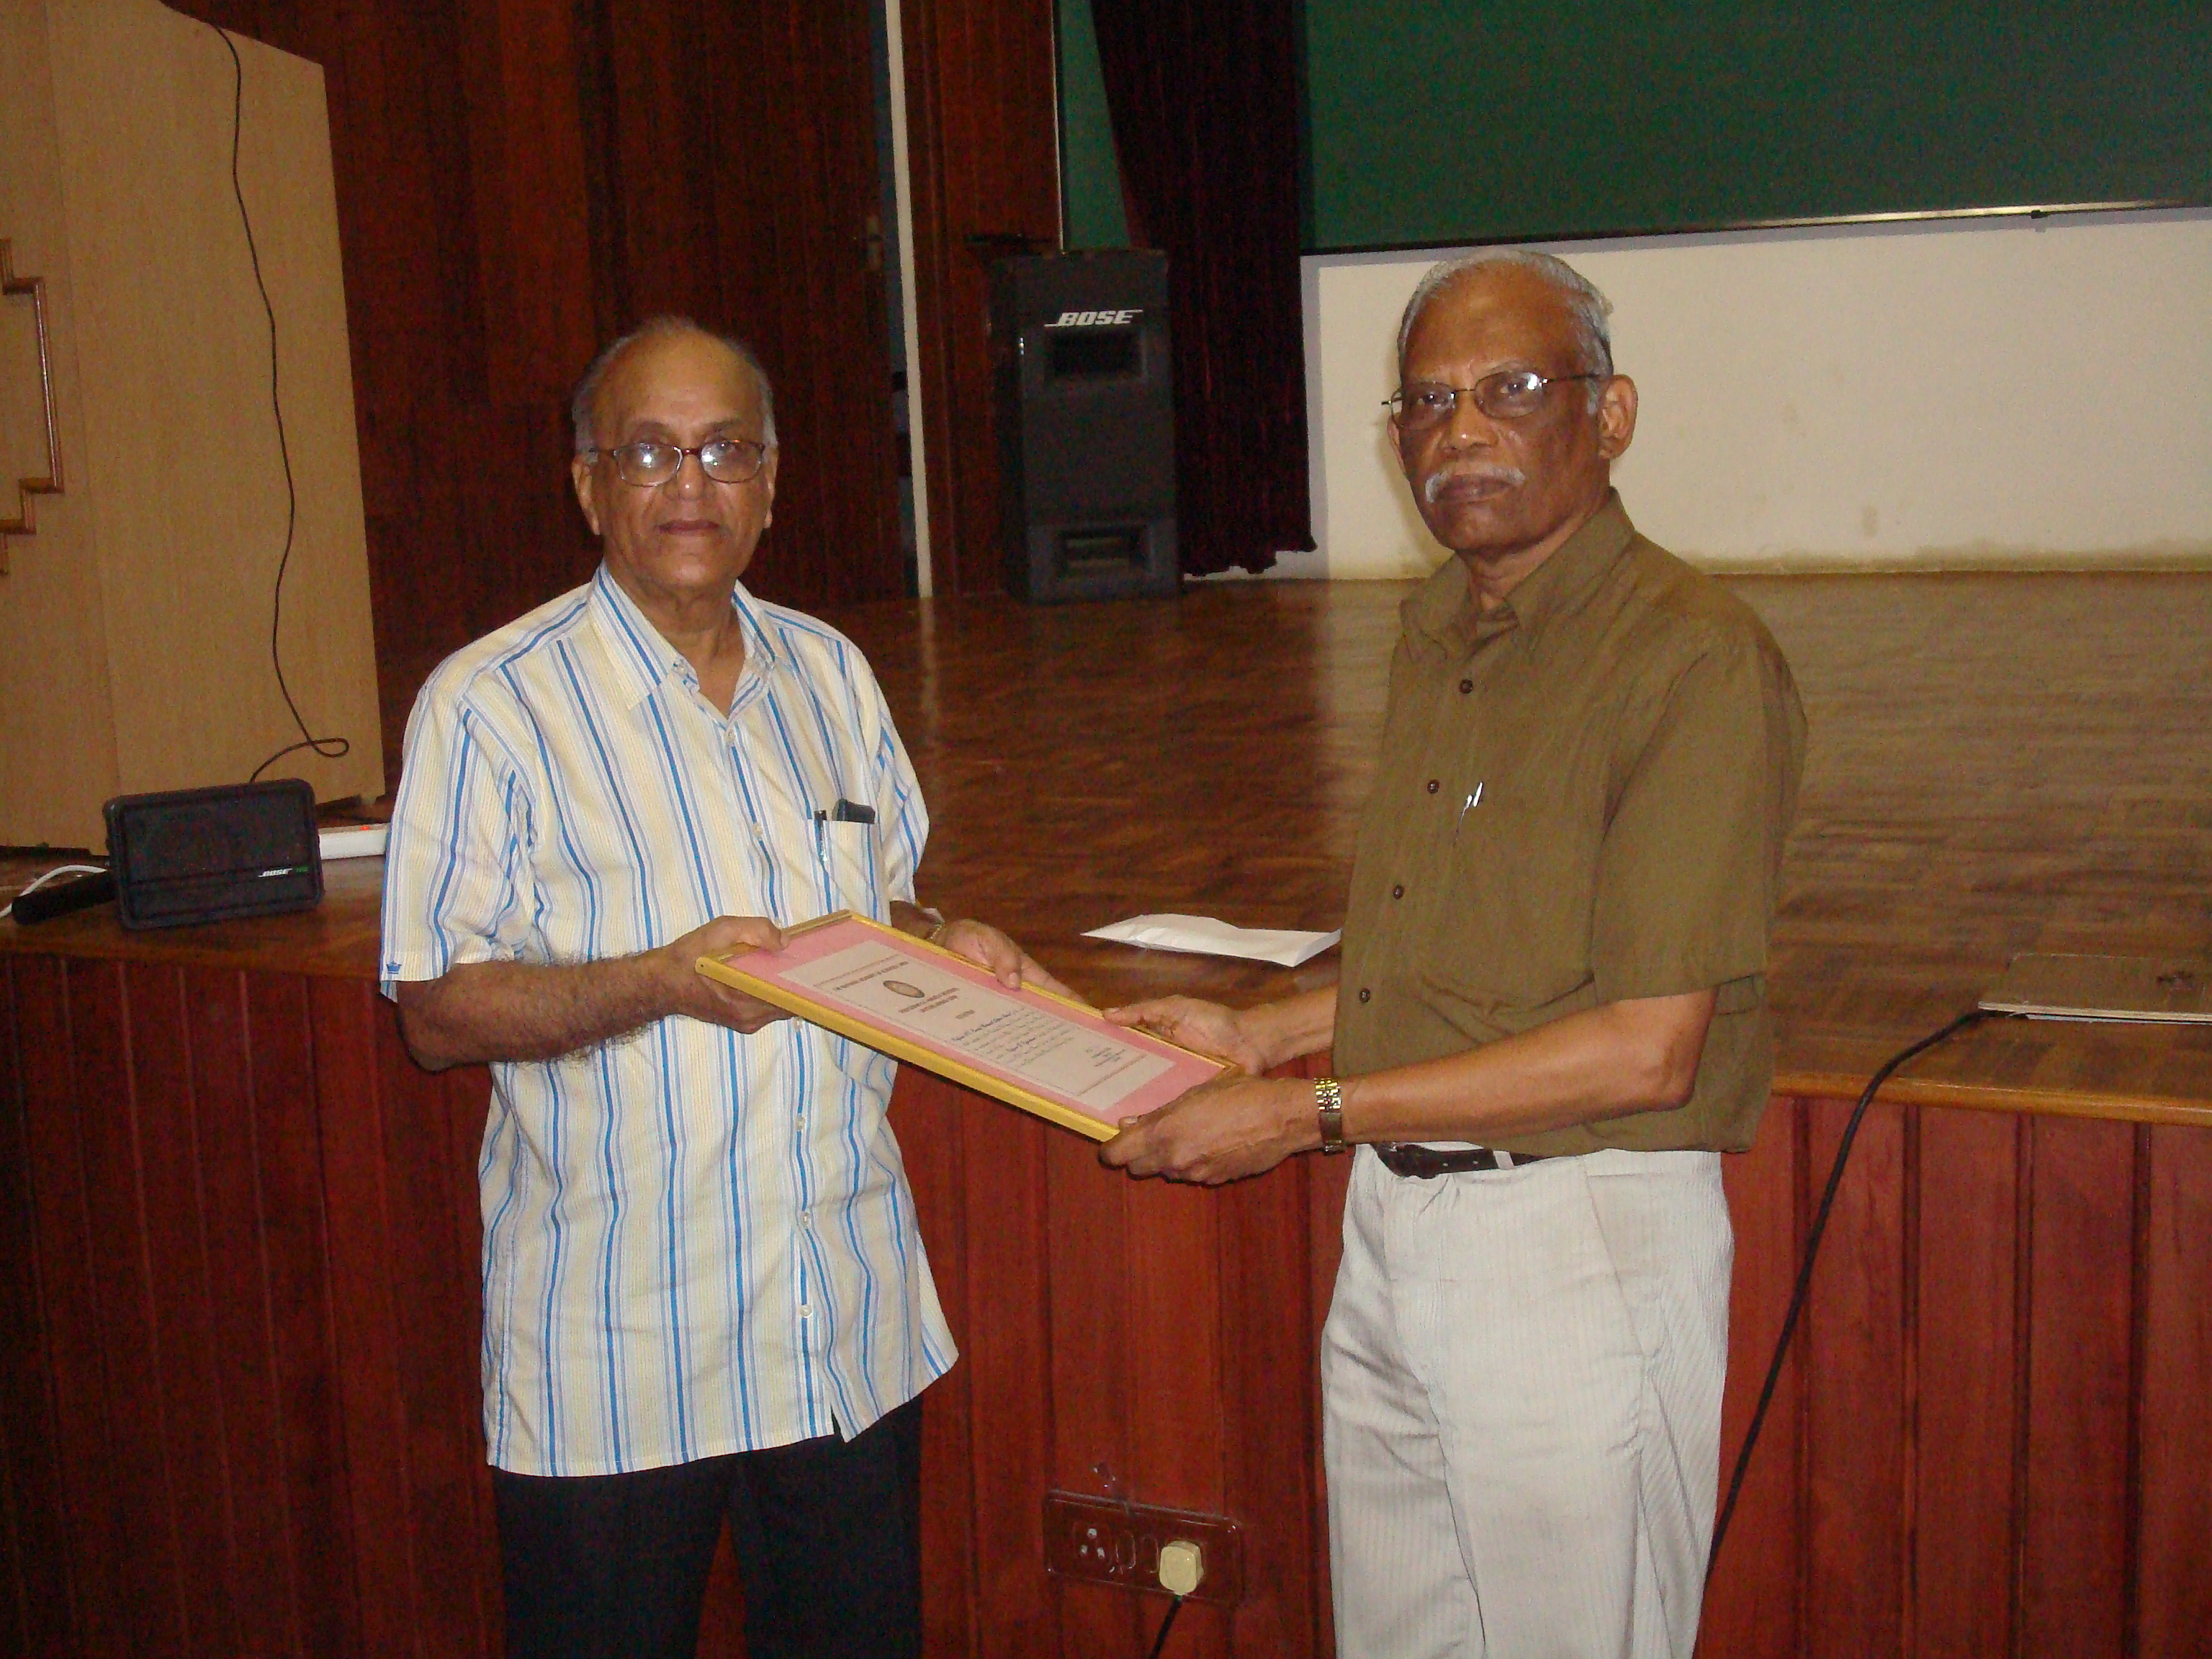
\includegraphics[width=0.8\textwidth]{images/Rajaji-seshadri.jpg}
\caption{\small{Receiving the A C Banerjee Memorial Award of The National\- Academy of Sciences from C S Seshadri, Director CMI.}}
\end{figure}

Some of the other institutions in whose development I played a role as a 
member of their Governing Council or other bodies are Harishchandra 
Research Institute, Institute of Physics, Saha Institute of Nuclear 
Physics, Inter-University Centre for Astro\-nomy and Astrophysics, SN Bose 
Centre for Basic Sciences, Indian\break Institute of Astrophysics and 
Astronomy and IISER, Thiruva\-nanthapuram.

\vspace{-\topsep}
\section*{Teaching}

Apart from teaching full courses at CMI, I have been involved in 
considerable teaching in other Centres too. Academies-organized 
Refresher Courses in many Colleges in Tamil Nadu, Kerala and Karnataka 
took up a lot of my time and energy. For many of them I was the 
Director. Sunday Classes (venue: Dept of\break Nuclear Physics of the 
University) were started by Satyanarayana of Pondicherry University with 
the help of Joseph Prabagar of Loyola College. I joined the team and 
taught. I was involved in the running and teaching in the DST-organized 
SERC Schools in Theoretical High Energy Physics for more than ten years 
and I initiated the Physics Teaching for Talented Students. Courses in 
High Energy Physics were given by me at IISER-Thiruvanantha\-puram, 
IISER-Mohali, Banaras Hindu University Madurai Kamaraj University and 
many other institutions.
\medskip

\begin{figure}[h]
\centering
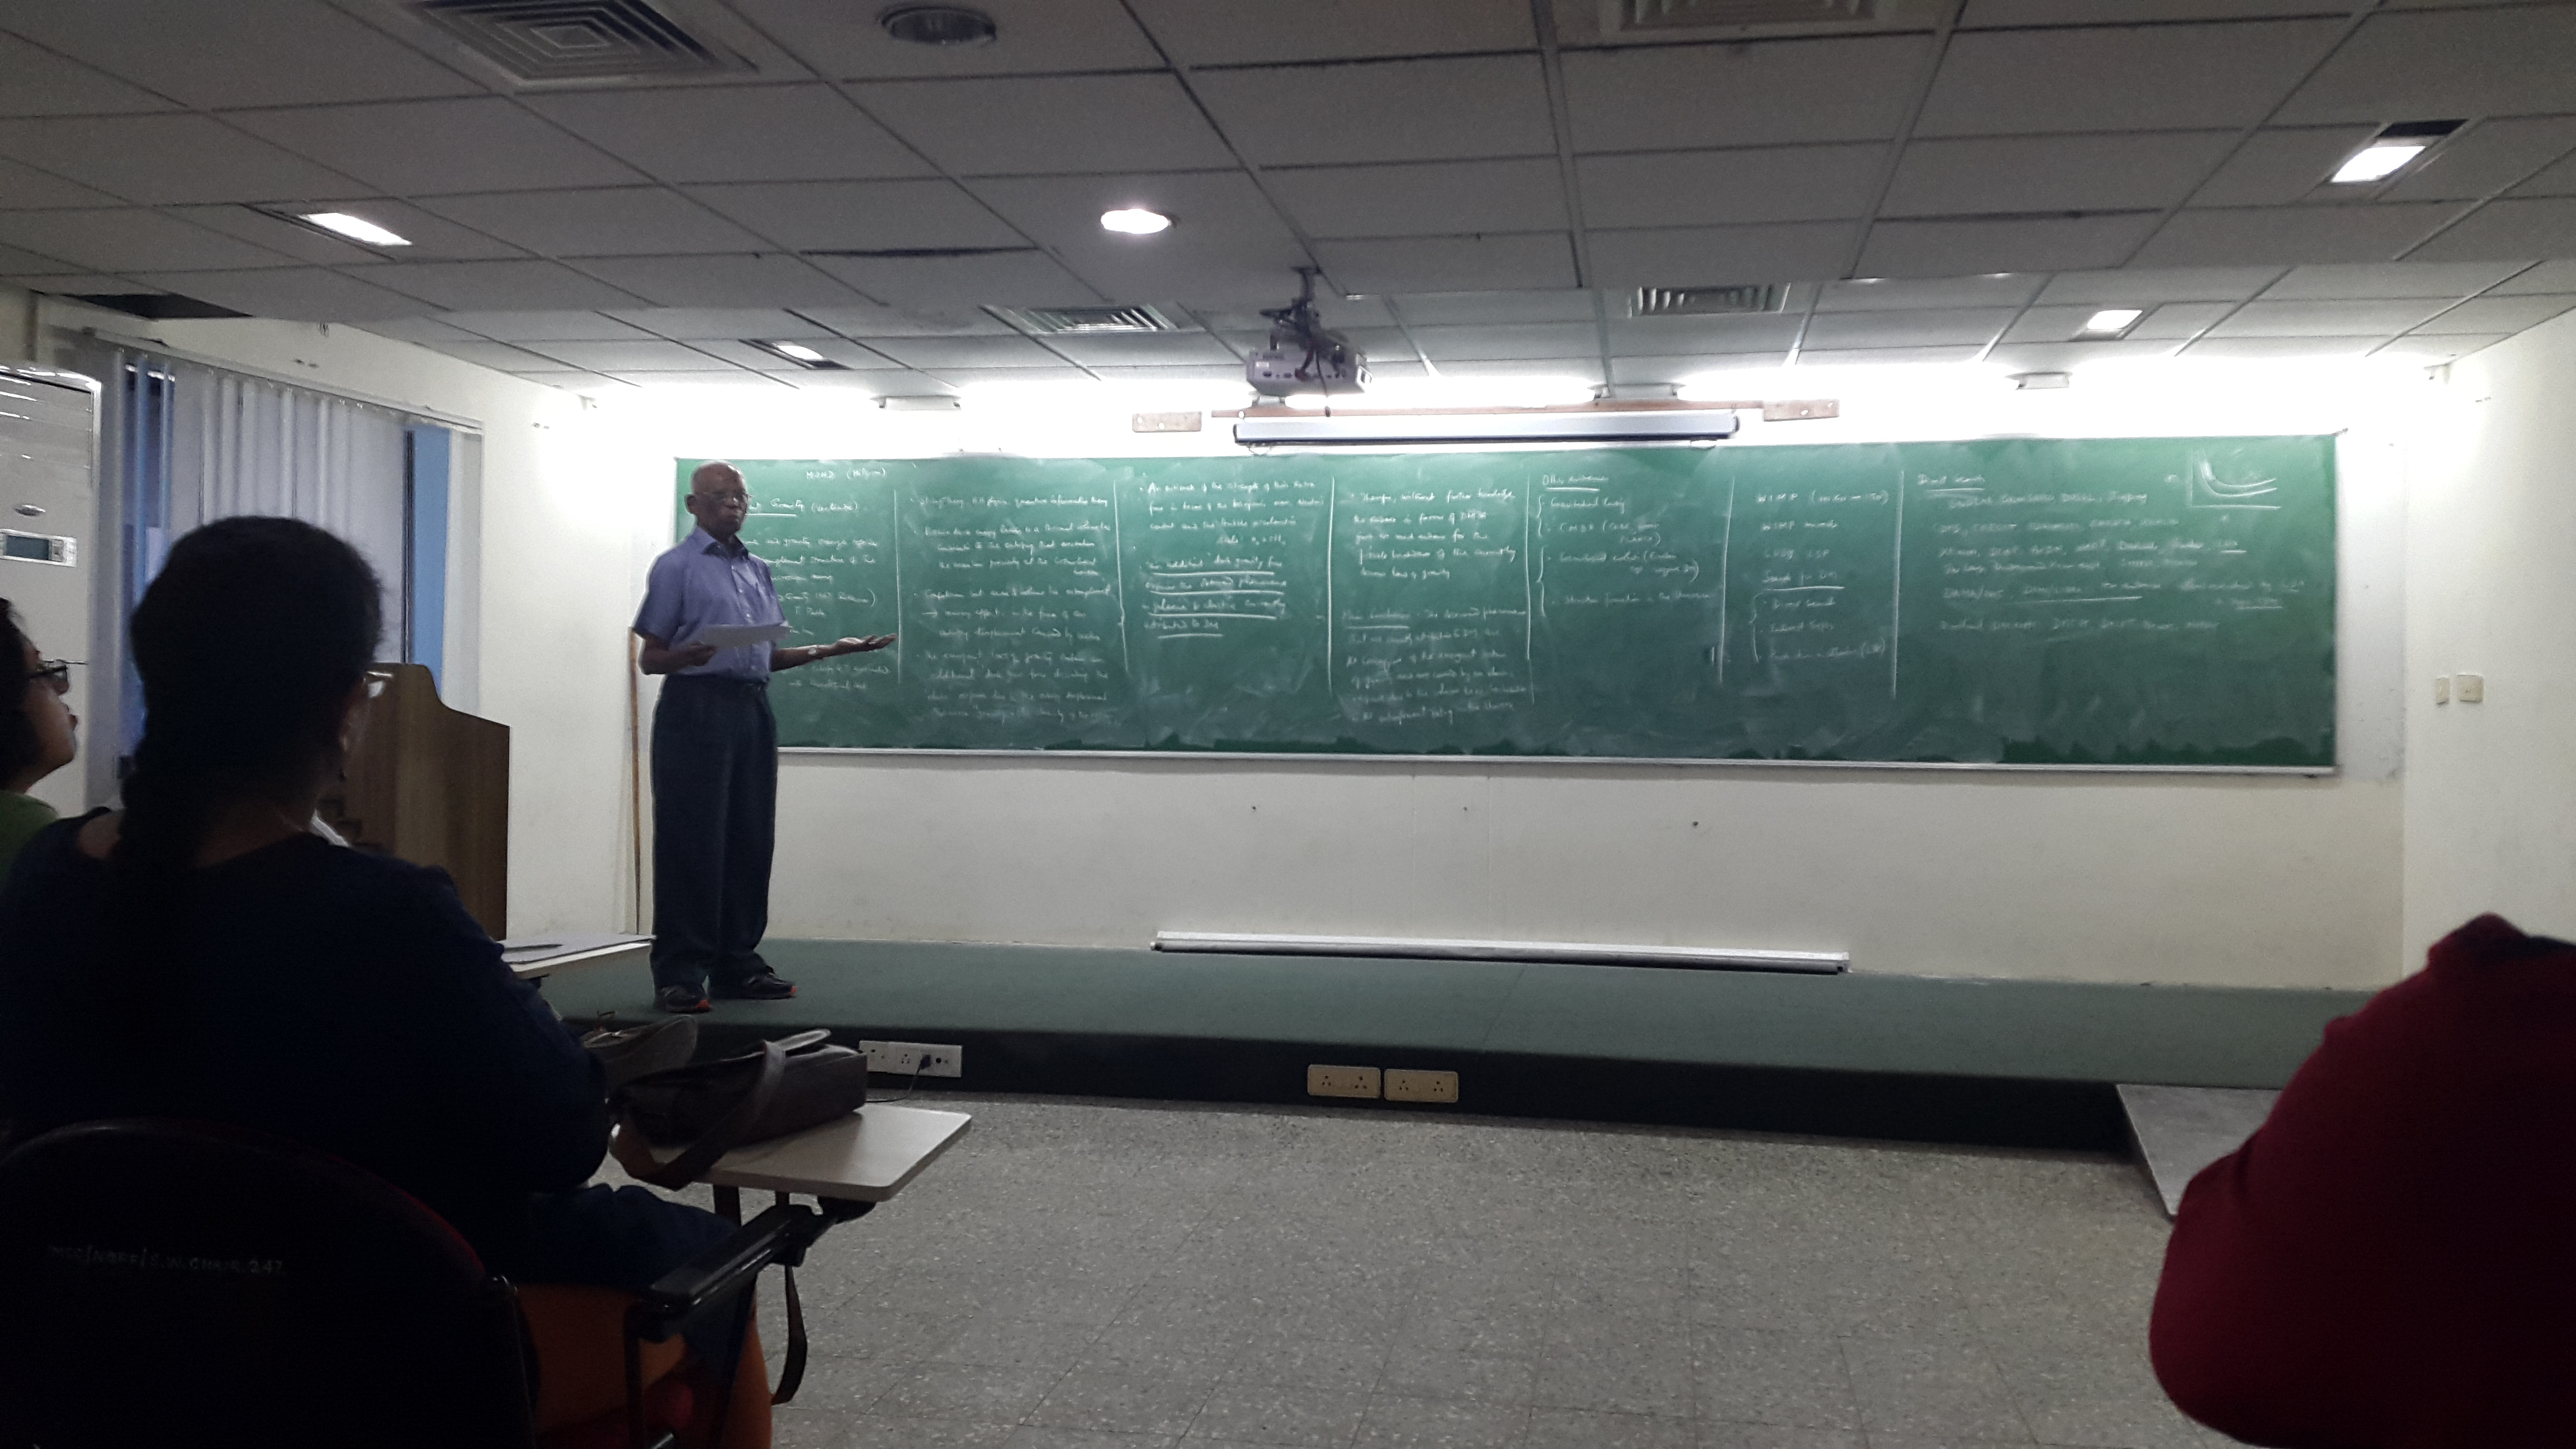
\includegraphics[width=\textwidth]{images/rajaji-teach1.jpg}
\caption{Lecturing at IMSc.}
\end{figure}
\newpage

\section*{Popular Science}

I strongly believe that Popular Science will succeed in the country
only if it is done 
in the mother tongue of the people. My ambition to write Science in Tamil 
fructified through the kindness of my friend Dr Jeyapragasam who was the 
Editor of a Tamil monthly published from Madurai. I wrote every month 
and brought out two volumes containing my articles.
\bigskip

\begin{figure}[h]
\centering
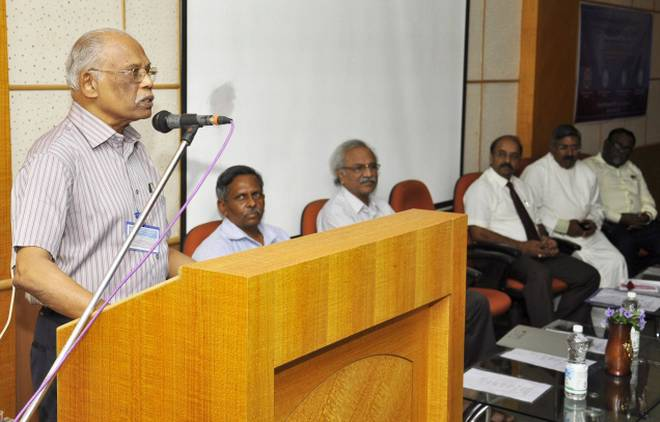
\includegraphics[width=\textwidth]{images/Rajaji-outreach-1.jpg}
\caption{At one of the Academy's Refresher School.}
\end{figure}
     
\section*{New Forms of Quantum Statistics}

AK Mishra and myself discovered many new forms of quantum statistics during
the period 1990 to 95. This was possible because of the Generalized Fock Space
that we constructed. Some of the new forms of statistics were Orthostatistics, 
Null Statistics and Hubbard Statistics. Along with this we constructed many
new algebras of creation and destruction operators. Many of these are expected
to be used in future, in String Theory and other fundamental theories.
\newpage

\section*{String Theory and LPA}

I was aware of String Theory almost from its birth. When I was perusing 
the preprint library in KEK, Japan in 1980 I saw the paper of Scherk and 
Shwartz who liberated String Theory from its hadronic context by 
changing the string tension from 1 GeV to $10^{19}$ GeV. That was the birth 
of String Theory. Then in 1984 I was escorting Tullio Regge from 
Bangalore to Madras and he told me the exciting discovery made by Green 
and Schwarz that all the anomalies cancel in the SO(32) and $E_8 \times E_8$ 
Superstring theories.

From then on I learnt whatever was known in String Theory and gave 
lectures on it in various Conferences, Workshops and the SERC School. 
But because of the heavy work involved in the building up of IMSc 
(1984-88) and the turmoil in 1989, I could not work in String Theory. 
But I kept up my interest in it because I believe that is the Theory for 
Future incorporating Standard Model and Quantum Gravity.

The main difficulty of String Theory is the lack of experimental 
support. That requires construction of accelerators going up to Planck 
energy $10^{19}$ GeV. Many regard that as impossible. This is a crisis in 
Physics. But human ingenuity knows no bounds and this energy barrier 
will be crossed. New principles of acceleration will be discovered. I 
have been emphasizing this for the last 40 years. Laser Plasma 
Acceleration (LPA) is one such and it has been pursued for some time all 
over the world. I have discussed the importance of starting LPA with 
experts on lasers at TIFR, Raja Ramanna Centre for Advanced Technology, 
Institute for Plasma Research and BARC. All of them met at the 
International Centre for Theoretical Sciences and they are chalking out 
a plan of action.

In the 80's I had many discussions with CVK Baba and MVN Murthy about 
building an accelerator of energy in the 5 to 10 GeV in India. DAE was 
willing to support it, but there was no enthusiasm among the 
experimental high energy physicists. They said such an accelerator would 
be useless unless it is more than 100 GeV. After this debate of ours, 
China built the Beijing storage ring of about 3 GeV which made many 
important contributions including a more precise measurement of tau mass 
which cleared many existing discrepancies.

Finally INDUS I and II were built after much delay but they were for 
synchrotron radiation.

Anyway, it is time that we now think of new methods of\break acceleration such 
as Laser Plasma Acceleration.

\vspace{-\topsep}
\section*{The contrast between the Indian situation pre-1971 and post-1984}

The success of the Standard Model based on YM theory has made YM a 
bandwagon. But I am talking about the pre-1971 era. As I already 
mentioned, I was lecturing on YM and electroweak theory in TIFR, SINP 
much before these things became popular, even before t'Hooft proved the 
renormalizability of YM with SBS. But there were no takers.

I remember, for instance, when I derived that in YM theory of weak and 
electromagnetic interactions the weak bosons have masses greater than 
37.4 GeV, many people jumped on my neck saying ``How can you put 
zero-mass photon and such heavy bosons in the same multiplet?". Times 
have changed. Now one routinely puts essentially ``zero-mass" particles 
and their superpartners, of TeV mass or even heavier, in the same 
supermultiplet.

When string theory came in 1984, there had arisen a suffici\-ently large 
number of capable young Indian physicists, both inside and outside the 
country who could pick up the new ideas fast and contribute at the front 
level.

It is clear that theoretical HEP in India has made rapid strides and now 
our theorists are equal to the best in the world.

\vspace{-\topsep}
\section*{Neutrinos}

Neutrino oscillations and neutrino mass were discovered during 
1996-2002. I was excited about Neutrino oscillations after I read about 
Mikheyev, Smirnow, Wolfenstein (MSW) effect in Bethe's PRL paper in 1986, 
that gave a beautiful explanation of MSW\break effect as a consequence of 
level crossing, during my visit to Hawaii in 1986. I conveyed that 
excitement to Anjan Joshipura and\break M V N Murthy who then wrote the first 
paper on three neutrino resonance phenomenon.

During the nineties,  MVN Murthy, D Indumathi, S Umasankar, 
Mohan Narayan and myself did considerable amount of work on neutrino 
phenomenology. We were the first to analyze all the\break neutrino data in a 
three-neutrino framework instead of the toy model using two neutrinos 
that was used until then. We were the first to analyze the null result 
of the CHOOSE reactor experi\-ment on the basis of the three-neutrino 
framework and get an upper bound on the $\theta_{31}$ angle to be 12 degrees. 
Later experiments showed this angle to be 9 degrees, close to our upper 
bound.

I also worked on models of neutrino masses and mixing in\break collaboration 
with Ernest Ma of the University of California,\break Riverside. One of the 
models that we constructed, the $A_4$ model, became quite popular.

In collaboration with MK Parida and Rabi Mohapatra, I\break discovered the 
real reason for the neutrino mixing angles to be different from the 
quark mixing angles and so large. It is the renormalization group 
evolution. Both the leptonic and quark mixing angles are of the 
Wolfenstein form at high scale and the leptonic angles alone get 
magnified at low scale.

\vspace{-\topsep}
\section*{Raju Raghavan}

Raju Raghavan was a great experimental physicist. Although I\break knew him 
earlier since he was a second batch trainee, we became\break friends only 
after I came to Madras. He used to visit me whenever he came from USA 
and we discussed neutrinos. He had many origi\-nal ideas on neutrino 
detection, including Mossbauer\break resonance absorption and emission of 
neutrinos. If one succeeds in this, neutrino experiments can be done on 
a table-top!
 
Later, after INO was conceived he was its enthusiastic promo\-ter. He had 
conceived a detector of solar low energy neutrinos, called LENS (Low 
Energy Neutrino Spectrometer) which can\break revolutionize solar neutrino 
physics. He wanted to do the experi\-ment in India. I took him to meet the 
secretaries of DAE and DST and they agreed to support him.

But Raghavan passed away suddenly in 2011. I was shocked and took a long 
time to recover. Actually at that moment when I heard the news, I was 
arranging a major meeting of Raghavan with scientists and science 
administrators. His death is a serious loss to Indian Science. India 
must take up the LENS Project.
\newpage

\section*{India-based Neutrino Observatory (INO)}

India was a pioneer in neutrino experiments. The very first obser\-vation 
of cosmic ray produced neutrinos called atmospheric\break neutrinos was made 
in India, in the Kolar Gold Field (KGF) mines. That was in 1965. But the 
mines were closed in the 90's. Since there was not much gold, the 
Bharath Gold Mines company decided to close it. We should not have let 
that happen. ``Science is more precious than gold."
\medskip

When the issue of possible closure of the KGF mines came up, I argued in 
favour of keeping them alive for future underground experiments. I 
raised it in many meetings. In the DST meeting on Thrust Areas held at 
Santiniketan, MVN Murthy presented both the issues, the case for keeping 
the KGF and construction of an accelerator for HEP.
\medskip

It was neccessary to spend some money for keeping the water in the mines 
out by pumping. But that is negligible compared to the cost of digging 
new tunnels. If this had been done, there would have been a continuity 
in Indian neutrino experiments from Kolar to INO.
\medskip

It is the atmospheric neutrinos which in the hands of the Japanese 
physicists enabled them to get two Nobel Prizes, in 1998 and 2002. We 
clearly missed the boat.
\medskip

Can we recover this lost initiative? We can and we must. The INO was 
conceived with this aim in view.
\medskip

It was conceived in IMSc in the year 2001, but it has not still seen the 
light. It was approved by all the Central Government bodies and the 
Government granted Rs 1600 crores for the project. This involves the 
construction of a 50, 000 ton magnetised iron calorimeter detector for 
atmospheric neutrino studies. This will be installed inside a mountain 
in Theni District. The nerve-centre of INO will be in the outskirts of 
Madurai City and will house R and D of particle detectors with training 
facilities for students. This has been named Inter-Institutional Centre 
for High Energy Physics (IICHEP).
\medskip

Apart from the study of atmospheric neutrino oscillations,\break INO lab will 
house experiments searching for Neutrinoless\break Double Beta Decay (NDBD) 
and Dark Matter (DM). CVK Baba and myself played some role in initiating 
the NDBD activity. As a consequence two or three groups involving 
Vandana Nanal, RG Pillay, PK Raina and PK Rath are involved in 
feasibility studies for the NDBD project. I tried to initiate work on 
Dark Matter Search through Rupak Mohapatra of Texas A and M and 
physicists at SINP. This could have been a major project but it did not 
succeed. Instead a minor Dark Matter project at a shallow depth in the 
Jaduguda mines has been started.
\medskip

\begin{figure}[h]
\centering
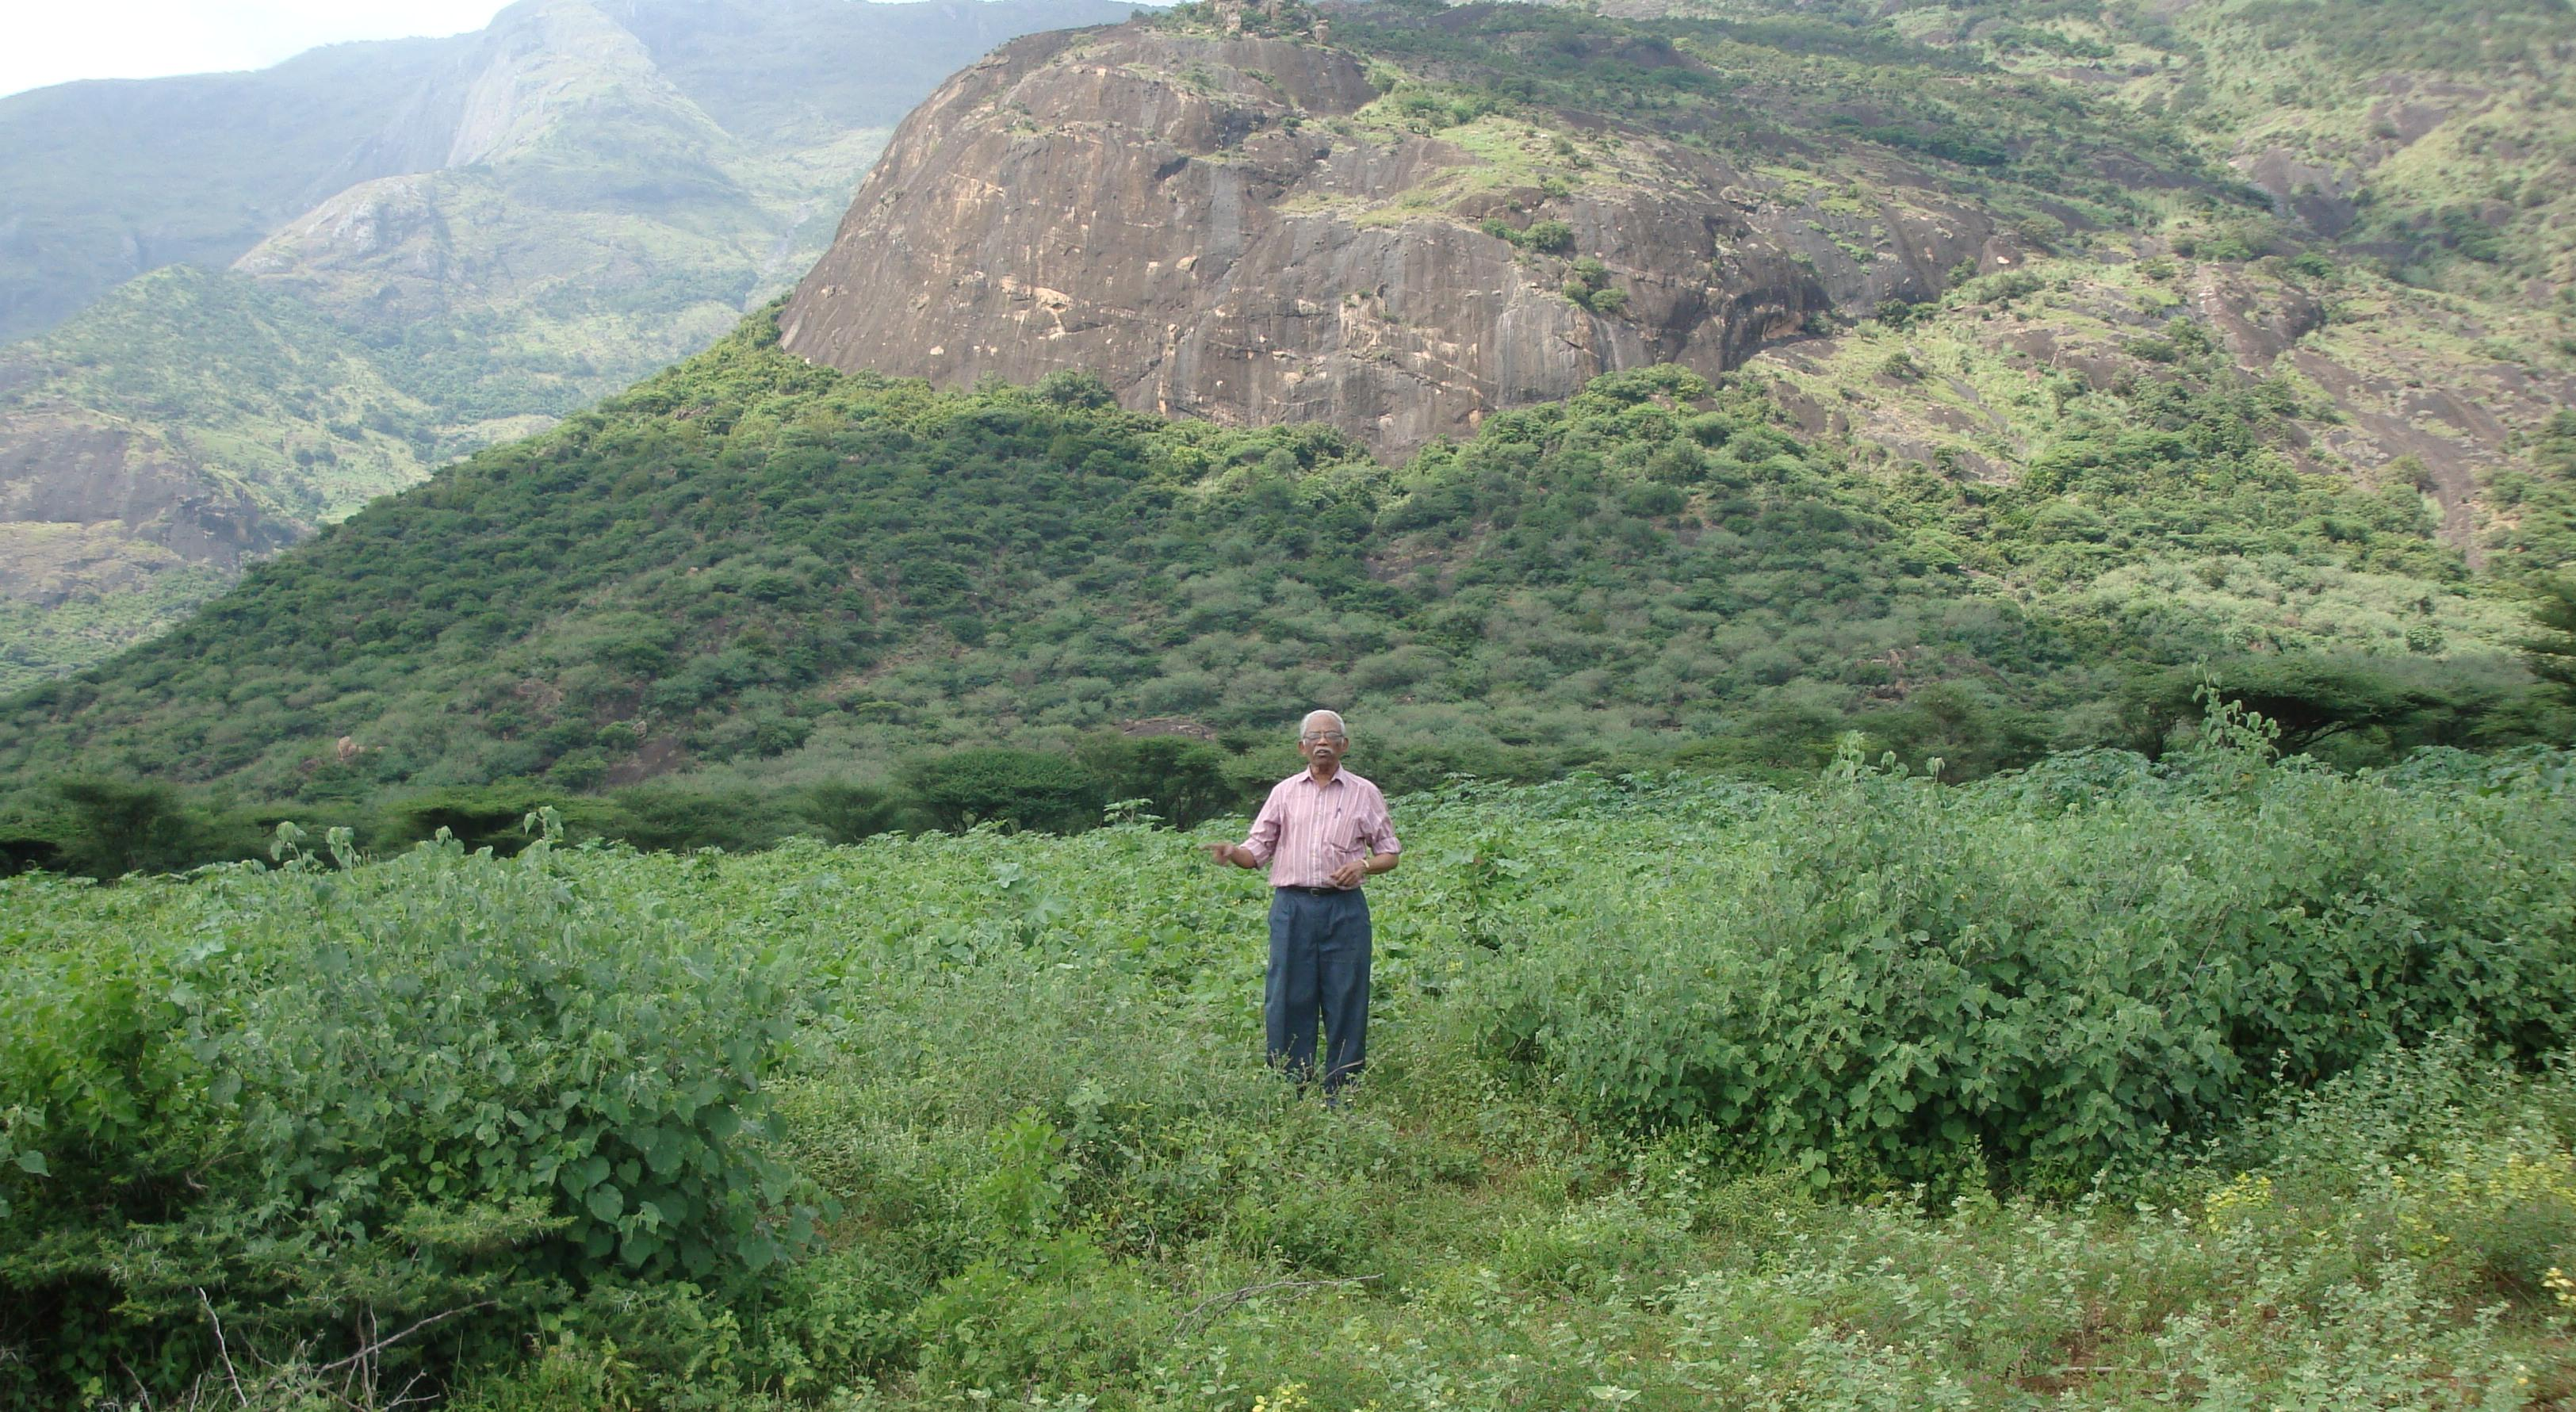
\includegraphics[width=\textwidth]{images/Rajaji-ino.jpg}
\caption{At the site in Theni District chosen for INO.}  
\end{figure}
\smallskip

Along with others I have lectured on INO to students in\break colleges and 
schools and villagers as a part of of the INO's outreach programme. This 
is continuing.
\medskip
  
Some ``wise men" of Tamil Nadu blocked INO citing\break non-existent 
environmental and other imaginary dangers. This\break obscurantist propaganda 
must be fought and INO must succeed. Truth has to triumph.

\vspace{-\topsep}
\section*{Family}

I have been blessed with a loving family - Suthandra Devi (my wife), 
Poongodhai and Uma (my daughters), Sunil Ramachandran (Poongodhai's 
husband), James Harano, (Uma's husband), Anjali and Shalini 
(Poongodhai's daughters) and Kailash (Uma's son).
Along with my family there are many friends who supported me, too 
numerous to mention by name.
\bigskip

\begin{figure}[h]
\centering
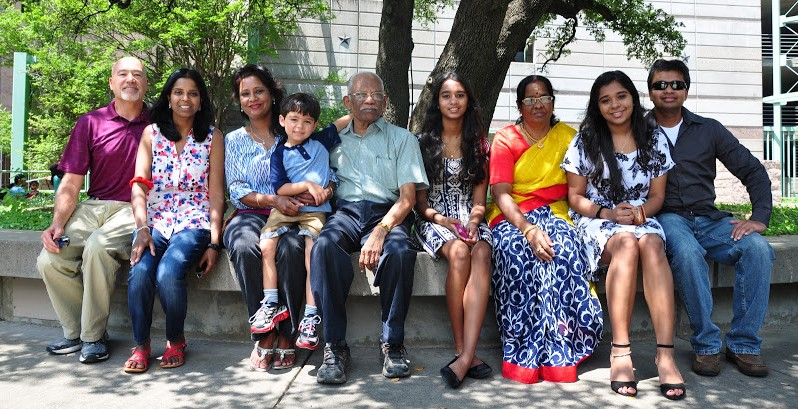
\includegraphics[width=\textwidth]{images/Rajaji-family-1.jpg}
\caption{Circa 2017 L to R: James, Uma, Poongodhai, Kailash, GR, 
Shalini, Suthandra, Anjali, Sunil.}
\end{figure}

